\sectionquestion{$K$-Means}

\begin{parts}

\part Suppose we wish to apply $K$-Means to the unlabeled 2D dataset $\Dc = \{ \xv^{(i)} \}_{i=1}^N$ below.

\begin{center}
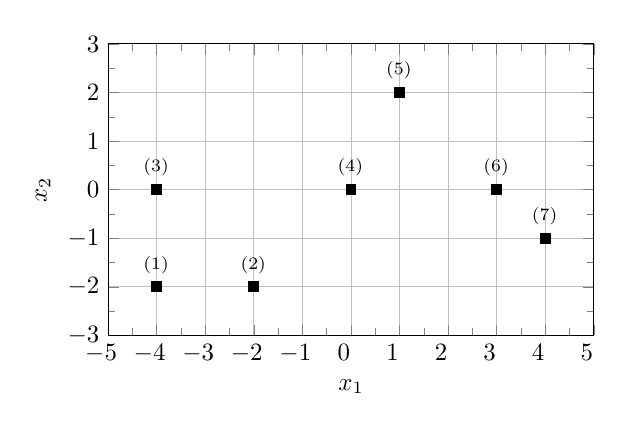
\begin{tikzpicture}[thick,scale=0.9, every node/.style={transform shape}]
    \begin{axis}[
        axis equal image,
        xmin=-5, xmax=5, xtick={-5,...,5},
        ymin=-3, ymax=3, ytick={-3,...,3},
        xlabel={$x_1$}, ylabel={$x_2$},
        samples=50, grid=major, minor tick num=1,
        xticklabel style={xshift=-0.1cm}]
      \addplot [
            scatter,
            only marks,
            point meta=explicit symbolic,
            scatter/classes={
                a={mark=square*,black}
            },
            nodes near coords*={$\xv^{(\pgfmathprintnumber[frac]\myvalue)}$},
            visualization depends on={\thisrow{myvalue} \as \myvalue},
        ] table [meta=label] {
            x y label myvalue
            -4 -2 a 1
            -2 -2 a 2
            -4 0 a 3
            0 0 a 4
            1 2 a 5
            3 0 a 6
            4 -1 a 7
        };
    \end{axis}
\end{tikzpicture}
\end{center}
 
We set $K=3$ and initialize the cluster centers to $\xv^{(4)}, \xv^{(5)}, \xv^{(7)}$. 
(Assume a single iteration first computes cluster assignments and then computes cluster centers.) 

\begin{subparts}

    \subpart[2] \textbf{Short answer:} What will the partitioning of the points be after the \textbf{first} iteration of $K$-Means? 

        cluster 1: \hspace{3.2cm} cluster 2:  \hspace{3.2cm} cluster 3: 
                
        \begin{tcolorbox}[fit,height=1cm, width=4.5cm, blank, borderline={1pt}{-2pt},nobeforeafter]
        %solution
        \end{tcolorbox}
        \hspace{1em}
        \begin{tcolorbox}[fit,height=1cm, width=4.5cm, blank, borderline={1pt}{-2pt},nobeforeafter]
        %solution
        \end{tcolorbox}
        \hspace{1em}        
        \begin{tcolorbox}[fit,height=1cm, width=4.5cm, blank, borderline={1pt}{-2pt},nobeforeafter]
        %solution
        \end{tcolorbox}
        
        \begin{soln}
        The rubric here should almost certainly NOT be a simple binary check of whether each cluster is correct. That is, there will probably be only a small number of wrong answers and we should group those into equivalence classes.
        
        cluster 1: $\xv^{(1)}, \xv^{(2)}, \xv^{(3)}, \xv^({4})$\\
        cluster 2: $\xv^{(5)}$\\
        cluster 3: $\xv^{(6)}, \xv^{(7)}$\\
        \end{soln}
        \begin{qauthor}
        Matt
        \end{qauthor}

    \subpart[2] \textbf{Short answer:} What will the partitioning of the points be after the \textbf{second} iteration of $K$-Means?

        cluster 1: \hspace{3.2cm} cluster 2:  \hspace{3.2cm} cluster 3: 
                
        \begin{tcolorbox}[fit,height=1cm, width=4.5cm, blank, borderline={1pt}{-2pt},nobeforeafter]
        %solution
        \end{tcolorbox}
        \hspace{1em}
        \begin{tcolorbox}[fit,height=1cm, width=4.5cm, blank, borderline={1pt}{-2pt},nobeforeafter]
        %solution
        \end{tcolorbox}
        \hspace{1em}        
        \begin{tcolorbox}[fit,height=1cm, width=4.5cm, blank, borderline={1pt}{-2pt},nobeforeafter]
        %solution
        \end{tcolorbox}
        
        \begin{soln}
        The rubric here should almost certainly NOT be a simple binary check of whether each cluster is correct. That is, there will probably be only a small number of wrong answers and we should group those into equivalence classes.

        cluster 1: $\xv^{(1)}, \xv^{(2)}, \xv^{(3)}$\\
        cluster 2: $\xv^({4}), \xv^{(5)}$\\
        cluster 3: $\xv^{(6)}, \xv^{(7)}$\\
        \end{soln}
        \begin{qauthor}
        Matt
        \end{qauthor}

    \subpart[1] \textbf{Short answer:} How many total iterations will complete before $K$-Means has converged? (We say that $K$-Means has converged if the next iteration, the cluster assignment will not change.)
        \begin{tcolorbox}[fit,height=1cm, width=4cm, blank, borderline={1pt}{-2pt}]
        %solution
        \end{tcolorbox}        
        \begin{soln}
        2
        \end{soln}
        \begin{qauthor}
        Matt
        \end{qauthor}

\end{subparts}

\part[1] \textbf{True or False:} Given a fixed set of initial cluster centers, $K$-Means \emph{always} converges to the same final cluster assignment, assuming ties in distance are always broken the same way.

    \begin{checkboxes}
     \choice True 
     \choice False
    \end{checkboxes}
    \begin{soln}
    True
    \end{soln}
    \begin{qauthor}
    Matt -- Note for future semesters: We should have labeled the points A, B, C, D,... for easier reading when grading. Also if we had one box for each point and we asked students to simply label them with cluster IDs, then we could auto-grade with Hamming loss.
    \end{qauthor}

\begin{comment}
\part[1] \textbf{True or False:} $K$-Means++ initialization strategy never selects an outlier point as initial cluster centers.

    \begin{checkboxes}
     \choice True 
     \choice False
    \end{checkboxes}
    \begin{soln}
    False
    \end{soln}
    \begin{qauthor}
    Matt
    \end{qauthor}
\end{comment}

\end{parts}